\begin{figure}[h]
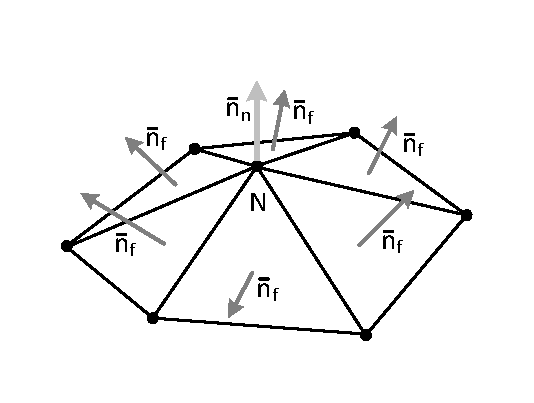
\includegraphics[width=0.48\textwidth]{pics/pic_architecture_size.pdf}
\captionstyle{center}\caption{Архитектура расчетной сетки.}\label{fig:pic_architecture}
\end{figure}

Решение задачи перестроения поверхности будем рассматривать на неструктурированной поверхностной расчетной сетке.
Элементами расчетной сетки являются узлы ($N_i$), ребра ($e_i$)  и ячейки ($f_i$).
Для удобства каждый элемент сетки связан со всеми своими инцидентными элементами: так связаны между собой инцидентные узлы и ребра, узлы и ячейки, ребра и ячейки. Множество инцидентных узлов будем обозначать $\mathscr{N}$, множество инцидентных ребер будем обозначать $\mathscr{E}$, а множество инцидентных ячеек будем обозначать $\mathscr{F}$.

К расчетной сетке предъявляются следующие требования.
Во-первых сетка должна быть целостной, то есть каждое ребро имеет ровно два инцидентных узла, отсутствуют изолированные и висячие узлы, а также изолированные ребра.
Во-вторых, все ячейки должны представлять собой треугольники (это гарантирует, что ячейка является плоской, так как четыре и более произвольных узлов могут не лежать в одной плоскости).
И в-третьих, рассматриваются только замкнутые сетки, представляющие собой поверхности, то есть каждое ребро имеет ровно две инцидентные ячейки.

\begin{equation}
\begin{cases}
\forall N_i \Rightarrow \mathscr{E}(N_i) > 2, \mathscr{F}(N_i) > 2 \\
\forall e_i \Rightarrow \mathscr{N}(e_i) = 2 , \mathscr{F}(e_i) = 2 \\
\forall f_i \Rightarrow \mathscr{N}(f_i) = 3 , \mathscr{E}(f_i) = 3 \\
\end{cases}
\end{equation}

В качестве дополнения также будем требовать, чтобы сетка представляла собой двустороннюю поверхность, для каждой ячейки однозначно определена нормаль к поверхности $\vec{n}_f$.
Также никакие два узла сетки не совпадают и отсутствуют ячейки с нулевой площадью (так как это сделает невозможным вычислений нормалей).
Для узла сетки будем рассматривать понятие нормали к поверхности и определять эту нормаль как

\begin{equation}
\vec{n}_n(N_i) = \frac{1}{|\mathscr{F}(N_i)|} \sum_{f_i \in \mathscr{F}(N_i)}{\vec{n}_f(f_i)}
\end{equation}